\begin{figure}
  \centering
  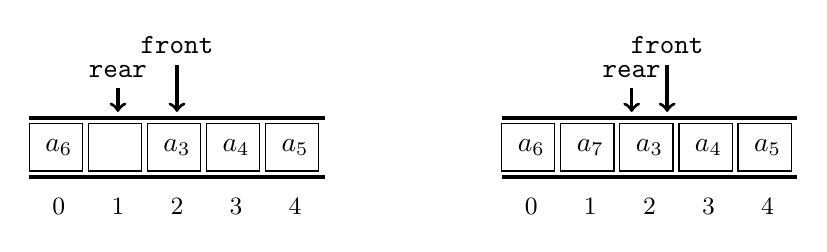
\begin{tikzpicture}
    \tikzstyle{information text}=[rounded corners,fill=blue!10,inner sep=1ex]
    \def\x{0.75}
    \def\y{0.75}

    \foreach \c in {0}{
      \ifthenelse{\c=0}{
        \def\r{0}
        \def\rr{0}
        \draw[very thick](\r*\x+\rr*\x,\c*\y)--(\r*\x+\rr*\x+5*\x,\c*\y);
        \draw[very thick](\r*\x+\rr*\x,\c*\y+\y)--(\r*\x+\rr*\x+5*\x,\c*\y+\y);        
        \foreach \r in {0,1,2,3,4}{                   
          \node[]at(\r*\x+\rr*\x+0.5*\x,\c*\y-0.5*\y){\small $\r$};
        }

        \foreach \r in {1,2,3,4,5}{         
          \draw[](\r*\x+\rr*\x-\x,\c*\y+0.1*\y)rectangle(\r*\x+\rr*\x-0.1*\x,\c*\y+0.9*\y);
        }
        \foreach \r in {3,4,5}{         
          \node[]at(\r*\x+\rr*\x-0.5*\x,\c*\y+0.5*\y){$a_{\r}$};
        }
        \def\r{3}
        \draw[->,very thick](\r*\x+\rr*\x-0.5*\x,\c*\y+1.9*\y)node[above]{{\tt front}}--(\r*\x+\rr*\x-0.5*\x,\c*\y+1.1*\y) ;
        \def\r{2}
        \draw[->,very thick](\r*\x+\rr*\x-0.5*\x,\c*\y+1.5*\y)node[above]{{\tt rear}}--(\r*\x+\rr*\x-0.5*\x,\c*\y+1.1*\y) ;
        \def\r{1}
        \def\rrr{6}
        \node[]at(\r*\x+\rr*\x-0.5*\x,\c*\y+0.5*\y){$a_{\rrr}$};

        %% %% %% %% %% %% %% 
        \def\rr{8}
        \draw[very thick](\rr*\x,\c*\y)--(\rr*\x+5*\x,\c*\y);
        \draw[very thick](\rr*\x,\c*\y+\y)--(\rr*\x+5*\x,\c*\y+\y);
        \foreach \r in {0,1,2,3,4}{                   
          \node[]at(\r*\x+\rr*\x+0.5*\x,\c*\y-0.5*\y){\small $\r$};
        }

        \def\rr{8}
        \foreach \r in {1,2,3,4,5}{         
          \draw[](\r*\x+\rr*\x-\x,\c*\y+0.1*\y)rectangle(\r*\x+\rr*\x-0.1*\x,\c*\y+0.9*\y);
        }
        \foreach \r in {3,4,5}{         
          \node[]at(\r*\x+\rr*\x-0.5*\x,\c*\y+0.5*\y){$a_{\r}$};
        }

        \def\r{3}
        \draw[->,very thick](\r*\x+\rr*\x-0.8*\x,\c*\y+1.5*\y)node[above]{{\tt rear}}--(\r*\x+\rr*\x-0.8*\x,\c*\y+1.1*\y) ;
        \draw[->,very thick](\r*\x+\rr*\x-0.2*\x,\c*\y+1.9*\y)node[above]{{\tt front}}--(\r*\x+\rr*\x-0.2*\x,\c*\y+1.1*\y) ;
        \def\r{1}
        \def\rrr{6}
        \node[]at(\r*\x+\rr*\x-0.5*\x,\c*\y+0.5*\y){$a_{\rrr}$};
        \def\r{2}
        \def\rrr{7}
        \node[]at(\r*\x+\rr*\x-0.5*\x,\c*\y+0.5*\y){$a_{\rrr}$};
        
      }
    }
  \end{tikzpicture}
\end{figure}
